In this chapter the summary of the project results will be summarized. Both applications which the final product consists of will be described and their main features together with the main limitations will be listed.  The functional and non-functional requirements will be reflected on so that it would be cleared that all of the project objectives were fulfilled. 

\section{Final product}
It was agreed with the customer that the final product would be split into to separate applications, the server-side and client-side part. Despite the fact the main responsibilities of the server (including processing the images and performing the detection, location and time synchronizations) represent computationally intensive tasks the customer insisted on implementing the server as a mobile application. The main reason is to enable the prospective power users or even developers to utilize the framework also for the other domains besides displaying imagery on the music concert crowd. The client-side on the other hand might be considered relatively simple application that only registers to the server and continuously changes the screen color according to the received textual commands.

\subsection{Server-side application}

\paragraph{Logic}
The server-side application is implemented in Java programming language using standard Google Android API and it supports the devices running on Android OS version 2.2 or higher. For the image processing module the Java version of OpenCV library was used and the networking is handled using the freely accessible library netlib. The time synchronization module uses the NTP time protocol and as an NTP server it uses the Android application Time server\footnote{\url{https://play.google.com/store/apps/details?id=com.icecoldapps.timeserver}} which must be downloaded and run prior to the server-side application. The application Digital Lighter Server can be downloaded through the online store Google Play\footnote{\url{https://play.google.com/store/apps/details?id=com.silentducks.digitallighterserver}}

For the detection the server uses the \textit{tree algorithm} as explained in Section \ref{txt:sprint5_immplementation} with the fallback option of linear \textit{one-by-one} algorithm. It can be chosen by the user how many colors should be used for the detection but the recommended value is three, specifically blue, white and red. The server is packed with a few images and animations of the various sizes and aspect ratios so that they could be played on the client devices right away.

\paragraph{GUI}
The graphical user interface should be as simple as possible as it only requires the user to set the server name, choose the number of colors for the detection and select the media to be played. GUI of the server can be seen in he Figure \ref{fig:Server_UI}.

\begin{figure}[H]
	\centering
		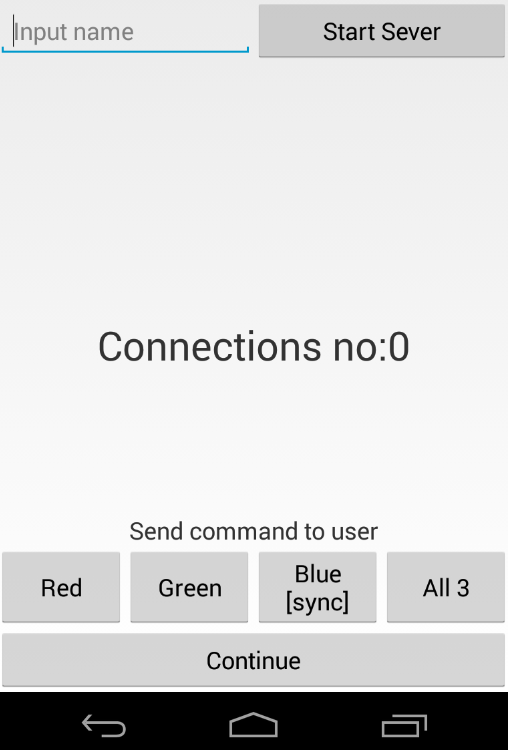
\includegraphics[width=5cm]{conclusion/server_ui.png}
	\caption{Server UI}
	\label{fig:Server_UI}
\end{figure}

\subsection{Client-side application}

\paragraph{Logic} 
As described in the introduction of this chapter the client application should be as simple as possible, so that it would run seamlessly on the wide range of Android phones and so that no user would come across any inconveniences preventing them from using the application. The client application only enables the user to choose one of the services that are offered on the local network and connect to them. From this point the client only waits for the signals to be continuously received from the server, parsing the textual protocol and responding to the single commands by changing the color of its screen.

The application Digital Lighter Client can be downloaded through the online store Google Play\footnote{\url{https://play.google.com/store/apps/details?id=com.silentducks.digitallighter}}.

\paragraph{GUI}
Similarly to the server-side application also the client GUI should be as simple as possible. The only task the user should perform is to manually select the offered service and connect. Then there is an option to hide the user interface buttons which can improve on the success rate of the detection. The GUI is depicted in the Figure \ref{fig:Client_UI}

\begin{figure}[H]
	\centering
		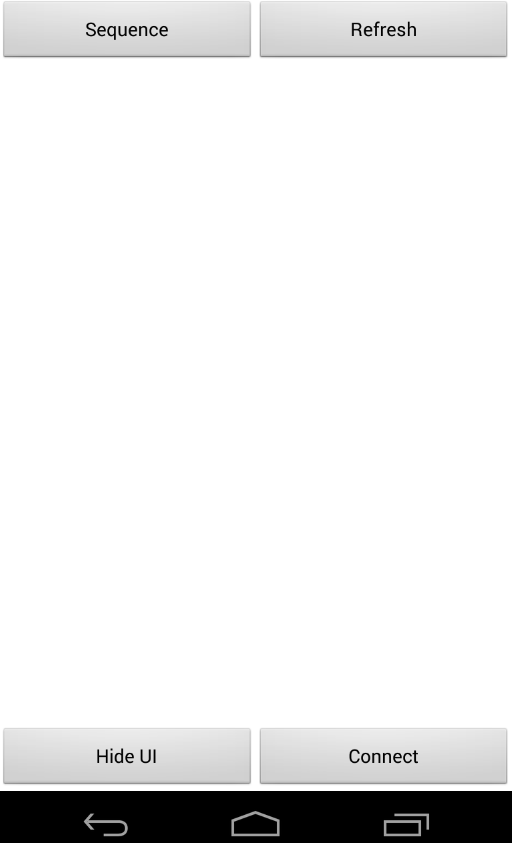
\includegraphics[width=7cm]{conclusion/user_ui.png}
	\caption{Client UI}
	\label{fig:Client_UI}
\end{figure}

%\subsection{Functionalities}
%As mentioned in Section \ref{txt:evaluation_customerandprojecttask} the customer confirmed the team managed to accomplish all given tasks. To prove this claim more formally both functional and non-functional requirements will be referenced with the description about how the certain task was accomplished.



\section{Limitations}
Though fully functioning the final product still suffers certain limitations and only works properly under certain constrained conditions. This is due to the fact the project represents proof of the concept product which mainly focuses on presenting the required features then scaling them for the real world conditions. The major limitations are as follows:

\paragraph{Limited FPS} The server is only able to display animations and videos with FPS\footnote{Frames Per Second} value not exceeding 5 FPS.

\paragraph{Limited detection color palette} The performance of the devices detection and location is influenced by what color is used for the detection. The experiments showed the combination of white, blue and red color gained best success ratio as stated in \ref{txt:evaluation_technicalissues}.

\paragraph{Dark environment} It is required that the client devices to be detected are placed in relatively dark environment so that the colors of their screens would contrast with the low ambient light.

\paragraph{Fixed position} After the detection is done the devices should not move more then in the range of the tile they were originally placed. This is due to the fact that device tracking was not implemented during this project as it was not considered that important task.

\section{Further work}
One of the main challenges for future is to improve the performance.
Higher FPS value would allow to display more interesting animations or even videos.
Also scalability in sense of number of client devices should be improved.

%___ DEVICE TRACKING ________________
\paragraph{Device tracking}
One of the first steps in further development is device tracking.
Once the mobile device is detected, its position is saved but not updated during time.
It is probable, that on rock concerts, the audience wont be static, but it will be in motion.
The current product would not be able to deal with that situation and the content would not be displayed properly.
One of the solutions might be to perform the initial detection and during playing the media it is known what color should each mobile device display and therefore the playing could be considered as a another continuous detection of devices.

%___ GRID ADJUSTING ________________
\paragraph{Grid adjustment}
Further work can also be focused on grid adjusting.
In non-artificial situations, it is possible, that the audience will be located only in the edge of the camera's snapshot.
The current prototype would not adjust to that situation, although it would be desired.
It would be adequate to keep the grid's dimension but to adjust the its resolution and position it to the edge, where audience is located.
One of the benefits of this extension is that the person who is controlling device with camera would not have to position and zoom it precisely.

%___ IMPROVE IMAGE PROCESSING  ________________
\paragraph{Improved image processing}
Even though device detection worked fine in dark environment, there are fields in which it could be improved.
The tree algorithm, described in Section \ref{subsec:tree_alg} will not work properly, when more devices are in the same tile.
Although there is a fallback algorithm, which will succeed in this case, its time complexity is too high for large audience.
Hence, a new algorithm with similar performance as the tree algorithm is desired.
Last but not least, if the detection worked even in worse light conditions it would significantly increased the potential of the product.

%___ SCREEN NOT PIXEL ________________
\paragraph{Extension of domain}
One of the interesting ideas for extension is not to display single color on a client device, which therefore works as a one pixel, but to display several pixels or even part of an image.
It would be possible to display complex images or videos even on few devices as can be seen in Figure \ref{fig:extension}.
This concept would required not only detection of position of devices but also finding its orientation.

\section{Summary}
During this project the mobile software product titled Digital Lighter was designed. It's main purpose is to entertain the audience of the music concerts and other social events who use their smartphones or tablets to participate in the huge human-screen.

The objective of the development team was to design and implement this application as well as manage the project using agile methodology Scrum, adapt to the requirements of the customer and deliver the extensive report summarizing the whole development process.

The team committed 1363 person-hours for all the project obligations and eventually it succeeded to deliver the working product which was approved of both customer and supervisor and submit the detailed report describing the development process.

%All team members from the development team, self-titled Silent ducks, collectively agreed the project was beneficial for them and that they learned new knowledge both from each other and from studying project related problematics. It should be therefore noted the team worked well together. Go team spirit.
